
\subsubsection{Computational Bioengineering }

\index{Roccatano, Danilo}

\paragraph{Research Team}
Danilo Roccatano (University Lecturer (Chemistry)) \\
The investigation of physico-chemical properties of 
biological  systems of industrial relevance using computational methods 
is one of the major aspects of  my research. I am interested in 
applying theoretical model and using molecular modelling to provide useful information
that drives enzyme evolution and protein engineering for biotechnological applications. Various aspects of my research activities are summarized below:
\begin{itemize}
\item Study of the effects of non-aqueous solvents and their water mixtures on the 
conformation, diffusive dynamics and reactivity of macromolecular systems for 
bioengineering. In particular, the solvent effect on 
protein folding and enzymatic activity is of high commercial and academic interest. 

\item In collaboration with Prof. U. Schwaneberg and collaborators, we are committed to 
developing computational tools to assist directed evolution experiments.~\cite{Wong06,Schenk06,Wong06b}
As a long term project, we are developing a Computational Bioengineering Portal (map.iu-bremen.de)
comprising various programs that assist random mutagenesis experiments. This publicly available server is dedicated to directed evolution community.   


\end{itemize}

\paragraph{Highlights}

Main research achievements in year 2006 are summarized as follow:

\begin{itemize}
 
\item{} The  collaboration with Prof. U. Schwaneberg and his PhD student T. S.
Wong resulted in two important achievements: 1) MD simulations study provided a clue on 
the mechanism of DMSO inactivation of heme monooxygenase P450 BM-3~\cite{Roccatano06a} (Fig. 1).  A subsequent 
resolution of the crystal structure of P450 BM-3 heme domain in 
presence of DMSO, performed by T. S. Wong in 
collaboration with Prof. M. Wilmanns at EMBL Hamburg, confirmed 
the theoretical hypothesis and showed the 
coordination of DMSO to the active site heme iron. 

\begin{figure}[ht]
  \begin{center}
    \includegraphics[width=6cm]{DrRoccatano-fig1.eps}
    \caption{ Snapshot of an MD simulation study of P450 BM-3 heme domain. The picture showed a DMSO molecule approaching the heme iron. }\label{fig:Roccatano1}
   \end{center}
\end{figure}

\item{}  Setting up a Computational Bioengineering Portal at Jacobs University (map.iu-bremen.de) (Fig. 2). 
The portal is dedicated to providing various computational 
support for directed evolution. It includes Mutagenesis Assistant Program (MAP)~\cite{Wong06,Schenk06} 
(running since beginning 2006, Fig. 2) that allows analyzing amino acid substitution patterns of 19 random mutagenesis methods upon input of a DNA sequence. Other two programs will be
available on the portal by the end of 2006, SeSaM-Tv and ExPoSeS. SeSaM-Tv is computational tool
to support Sequence Saturation Mutagenesis (SeSaM), a novel random mutagenesis method developed by T. S. Wong and Prof. U. Schwaneberg. ExPoSeS (Exploring Protein Sequence Space) provides guidance to efficiently explore protein sequence space using combinations of random mutagenesis methods.   

\begin{figure}[ht]
  \begin{center}
    \includegraphics[width=6cm]{DrRoccatano-fig2.eps}
    \caption{The Computational Bioengineering Portal at Jacobs University (map.iu-
bremen.de)}\label{fig:Roccatano2}
   \end{center}
\end{figure}


\end{itemize}

\nocite{Pal06,Roccatano06b,Sahoo06}

Danilo Roccatano is also involved in "Nano and Material Science".


\paragraph{Collaborations}
\begin{enumerate}
\item {\sl Jacobs University Bremen} \\ Prof. Ulrich Schwaneberg \\ Study of 
the organic solvent effects on
monooxygenase P450 BM-3 and Mutagenesis Assistant Program.
\item {\sl Jacobs University Bremen} \\ Prof. Werner M. Nau \\ Study of the 
dynamics in solution of small 
peptides by Molecular Dynamics simulation and time-resolved spectroscopic 
tecniques.
\item {\sl Jacobs University Bremen} \\ Prof. Martin Zacharias \\ Molecular 
Dynamics simulation study of the nucleosome core particle.
\item {\sl University of Salerno, Italy} \\ Dr. Giuseppe Milano \\ Interaction of 
polymer with biological membranes.
\item {\sl University of East Anglia, Norwich (UK)} \\ Dr. Steven Hayward \\ Theoretical 
investigation of domain motion in proteins.
\item {\sl Max Planck Institute for Biophysical Chemistry, Goettingen,Germany. } \\ 
Dr. Bert de Groot \\ Theoretical investigation of domain motion in proteins.
\end{enumerate}


